\documentclass{article}
\usepackage[utf8]{inputenc}
\usepackage[T1]{fontenc}
\usepackage{geometry}
\usepackage{graphicx}
\usepackage{multicol}

\geometry{margin=0.5in}

\begin{document}
\section*{Task}
\subsection*{\underline{Delaying Analog Signals Using Tables}}
Below is a basic block diagram of the system and the principle of delaying a quantized analog signal.

\begin{center}
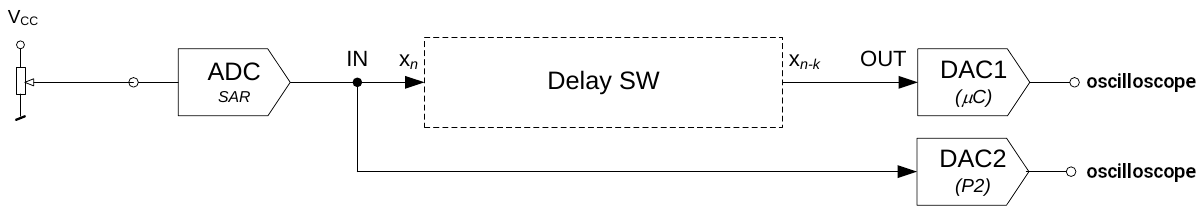
\includegraphics[width=\textwidth]{"../img/ADC_delay_DAC_1.png"} \\
Block Diagram of the Delay System \\
\vspace{5mm}
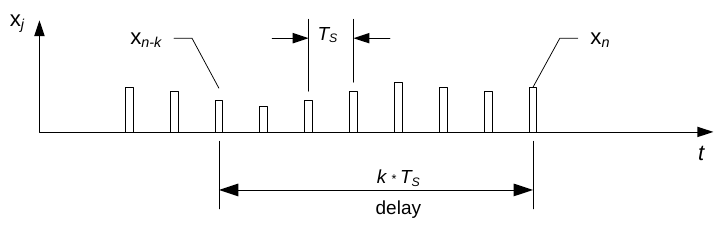
\includegraphics[width=0.7\textwidth]{"../img/ADC_delay_DAC_2.png"} \\
Samples \textbf{X\textsubscript{j}} of the analog signal \textbf{X}
\end{center}

The implementation of a FILO (First-In-Last-Out) register, which stores incoming samples and ensures the desired delay $k * T_s$ (where $T_s$ is the sampling period), can be done in various ways. Two approaches are outlined below:
\begin{itemize}
    \item consistently shifting the contents of memory cells forming the FILO register – not recommended
    \item placing the currently sampled data in a table and addressing the appropriate reading of the samples that were previously stored in the table. The principle of this method is shown below – the address for writing the currently sampled value and reading the delayed (previously entered) sample is incremented in each cycle. This ensures constant \textit{k}, and therefore a constant delay time.
\end{itemize}

\begin{center}
\noindent 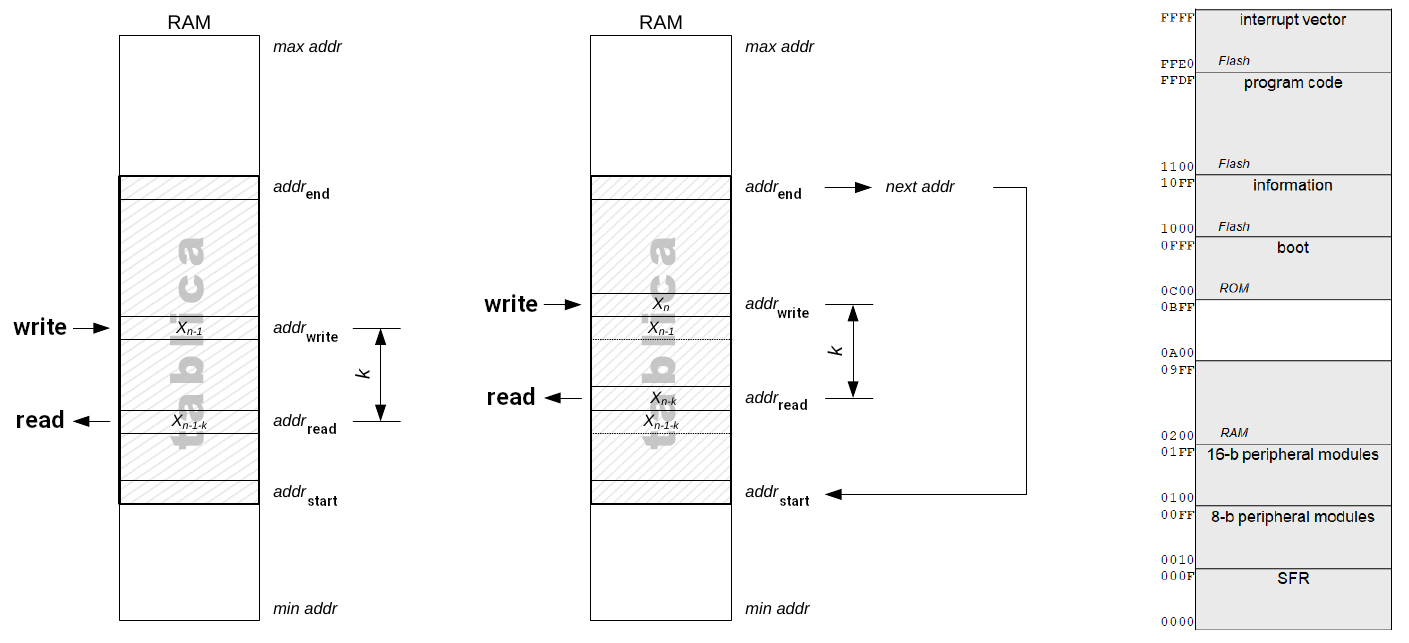
\includegraphics[width=0.9\textwidth]{../img/ADC_delay_DAC_3.png}
\end{center}

\begin{multicols}{3}
    \begin{center}
    \textit{n-1} moment (previous)
    \end{center}
    \columnbreak
    \begin{center}
    \textit{n} moment (current)
    \end{center}
    \columnbreak
    \begin{center}
    MSP430F169 memory map
    \end{center}
\end{multicols}

The table is placed in RAM and indirect addressing should be used for addressing it. When placing the table in the address range of RAM, \textbf{ensure there is no conflict with the area occupied by the \textit{stack}}.
\vspace{5mm}

Write a program to delay the analog signal:
\begin{itemize}
    \item delay in the range of 0.5–1.0 seconds
    \item the program should be implemented exclusively using interrupts from Timer\_A \\
    (\underline{not using the resources of the main program})
    \item suggested table size - 256 samples
\end{itemize}

\end{document}